%%%%%%%%%%    PREAMBLE    %%%%%%%%%%
\documentclass{article}

\usepackage{rotating}               % for the black border on side of screen
\usepackage{tikz}                   % graphic elements
\usepackage{fancyhdr}               % formatting headers and footers
\usepackage{titletoc}               % table of contents
\usepackage{graphicx}               % more graphics
\usepackage{caption}                % captioning graphics
\usepackage{url}                    % url references
\usepackage{float}                  % table trauma
\usepackage{placeins}               % forces figures to appear where they are defined
\usepackage{wrapfig}                % for wrapping text around figures 
\usepackage{colortbl}               % used for colouring aspects of floats
\usepackage{xcolor}                 % pretty colours?
\usepackage{geometry}               % page margins
\usepackage{hyperref}               % allows for hyperlinking
\usepackage{longtable}              % long table formatting
\usepackage{pgfgantt}               % for a gantt chart, currently unused
\usepackage{tabularx}
\usepackage{fontspec}
\usepackage{amsmath}
\usepackage{enumitem}
\usepackage{setspace}

\usepackage[fontsize=10.8pt]{fontsize}

\geometry{margin=2cm}
\setlength{\textfloatsep}{8pt}
\setlength{\floatsep}{6pt}
\setlength{\intextsep}{6pt}

\setmainfont{Times New Roman}

%%%%%%%%%%%%%%%%%%%%%%%%%%%%%%%%%%%%
\begin{document}
%%%%%%%%%%    COVER    %%%%%%%%%%
\begin{titlepage}
    \centering
    
    %-----------------------------------
    %  Lancs Uni Logo
    %-----------------------------------
    \vspace*{1cm}
    
\includegraphics[width=0.35\textwidth]{images/lancs-uni-logo.png}
    \vspace{1.5cm}
    
    %-----------------------------------
    % Document Title
    %-----------------------------------
    {\Huge \textbf{Software Design Document}}\\[1.2cm]
    
    {\Large Transport for North West}\\[1.5cm]
    
    %-----------------------------------
    % Module / Course Details
    %-----------------------------------
    \begin{spacing}{1.2}
    \large
    \textbf{Module Code:} SCC.200 \\[0.3cm]
    \textbf{Module Title:} Group Project \\[0.3cm]
    \textbf{Institution:} Lancaster University \\[0.3cm]
    \textbf{Department:} School of Computing and Communications
    \end{spacing}
    
    \vfill
    
    %-----------------------------------
    % Author Information
    %-----------------------------------
    \large
    \textbf{Group:} Group 5-2 \\[0.3cm]
    \textbf{Group Lead:} Rob Standen \\[0.3cm]
    
    \textbf{Members:} \\[0.2cm]
    \begin{tabular}{ll}
    Lance Villarin & Inhu Lee \\
    Jack Husband & Mike Sells \\
    \multicolumn{2}{c}{Matthew Oulton} 
    \end{tabular} \\
    
    \vspace{0.3cm}
    
    \textbf{Submission Date:} February 12, 2026
    
    \vspace{1cm}
    
\end{titlepage}
\newpage

%%%%%%%%%%%%%%%%%%%%%%%%%%%%%%%%%%%%%%%%%%%%
%%%%%%%%%%    LIST OF CONTENTS    %%%%%%%%%%
\tableofcontents
\newpage

%%%%%%%%%%%%%%%%%%%%%%%%%%%%%%%%%%%
%%%%%%%%%%    CONTENT    %%%%%%%%%%

\section{Executive Summary}
Currently, the north west of England is served by multiple transport operators, each maintaining independent timetables and journey-planning systems. These systems operate largely in isolation, making it difficult for users to plan journeys that involve multiple operators or modes of transport. The resulting complexity disproportionately affects infrequent users, visitors, and residents of rural or poorly connected communities. \\

Although a number of commercial journey-planning applications attempt to aggregate transport information across operators, such solutions often introduce additional limitations. These may include financial costs to operators or users, the presence of intrusive advertising, or incomplete coverage that excludes smaller operators delivering socially necessary services. \\

In response to these challenges, this document sets out the rationale and requirements for an integrated transport application designed to provide comprehensive, reliable, and user-centred journey planning across the region. The proposed system seeks to unify transport data from all relevant operators, support robust and accessible route selection, and contribute to a more coherent and attractive public transport network for residents and visitors alike.

%%%%%%%%%%%%%%%%%%%%%%%%%%%%%%%%%%%%%%%%%%%%%%%%%%%
%%%%%%%%%%%%%%%%%%%%%%%%%%%%%%%%%%%%%%%%%%%%%%%%%%%

\section{Scope}
This subsection defines the scope of the proposed integrated transport journey-planning system. It specifies the functional capabilities, and geographic coverage included within the project, as well as explicit exclusions and constraints. The scope establishes clear boundaries for system development and provides a precise definition of the project’s intended deliverables.

\subsection{In-scope}
\begin{itemize}[itemsep=2pt, topsep=4pt, parsep=0pt]
    \item Development of an integrated journey-planning system covering all participating transport operators within the region.
    \item Support for multi-operator and multi-modal journey planning.
    \item Provision of near-real-time service information, where such data is made available by operators.
    \item Delivery of a user-facing interface designed to be accessible to infrequent visitors and non-regular users.
    \item Route planning functionality based on criteria including journey time, number of interchanges, walking distance, and service availability.
\end{itemize}

%%%%%%%%%%%%%%%%%%%%%%%%%%%%%%%%%%%%%%%%%%%%%%%%%%%%%%%%%%%%%%%%%%%%
%%%%%%%%%%%%%%%%%%%%%%%%%%%%%%%%%%%%%%%%%%%%%%%%%%%%%%%%%%%%%%%%%%%%

\subsection{Out-of-scope}
The following items are explicitly excluded from the scope of this project:
\begin{itemize}[itemsep=2pt, topsep=4pt, parsep=0pt]
    \item Ticket purchasing, fare payment, or revenue allocation between operators.
    \item Modifications to existing transport services, routes, or timetables.
    \item Ownership, management, or operation of transport services.
    \item Advertising-led functionality or commercial modification of transport data.
    \item Guarantees regarding data quality beyond that supplied by participating operators.
\end{itemize}

%%%%%%%%%%%%%%%%%%%%%%%%%%%%%%%%%%%%%%%%%%%%%%%%%%%%%%%%%%%%%%%%%%%%
%%%%%%%%%%%%%%%%%%%%%%%%%%%%%%%%%%%%%%%%%%%%%%%%%%%%%%%%%%%%%%%%%%%%

\subsection{Geographic Boundaries}
This project has been commissioned by the local authority responsible for the coastal region spanning \textbf{Preston} to \textbf{Lancaster}, including \textbf{Blackpool}, \textbf{the Fylde}, and \textbf{the Wyre} coastal areas. Coverage of this system is therefore geographically bound to this region.

%%%%%%%%%%%%%%%%%%%%%%%%%%%%%%%%%%%%%%%%%%%%%%%%%%%
%%%%%%%%%%%%%%%%%%%%%%%%%%%%We decided to split the database into 4 main tables: User, userSavedRoute, savedRoute and Routes. We did this to help separate data into meaningful sections as well as eliminate duplicated data wherever possible. This ensures whatever we produce will be smaller in size, making it more beneficial and less likely to be erroneous. %%%%%%%%%%%%%%%%%%%%%%%

\section{Technological Requirements}
This section defines the functional and non-functional requirements for the system.
The requirements are derived from the project brief and stakeholder needs and specify
\emph{what} the system must do, rather than \emph{how} it will be implemented.

%%%%%%%%%%%%%%%%%%%%%%%%%%%%%%%%%%%%%%%%%%%%%%%%%%%%%%%%%%
%%%%%%%%%%%%%%%%%%%%%%%%%%%%%%%%%%%%%%%%%%%%%%%%%%%%%%%%%%

\subsection{Functional Requirements}

\begin{table}[H]
\centering
\renewcommand{\arraystretch}{1.3}
\begin{tabular}{|p{1cm}|p{4cm}|p{12cm}|}
\hline
\textbf{ID} & \textbf{Name} & \textbf{Requirement Description} \\
\hline
FR1 & Multi-Modal Journey Planning &
The system shall allow users to plan journeys that combine multiple transport modes, including bus and rail services, across the supported geographic region. \\
\hline
FR2 & Multi-Operator Integration &
The system shall integrate timetable and live service data from all supported local bus operators and National Rail services, without preferential treatment of any operator. \\
\hline
FR3 & Timetable Information Access &
The system shall provide scheduled departure and arrival times for buses and trains at all supported stops and stations. \\
\hline
FR4 & Live Service Information &
The system shall display live service data, including delays, cancellations, and real-time vehicle locations where available. \\
\hline
FR5 & Disruption Detection and Handling &
The system shall detect service disruptions, including delays, cancellations, and temporary service restrictions, and shall adjust journey planning recommendations accordingly where available \\
\hline
FR6 & Route Search and Selection &
The system shall allow users to search for, view, select, and save available transport routes for a specified journey with basic sorting functionality and the ability to set time constraints\\
\hline
FR7 & Geographic Visualisation &
The system shall present transport routes, stops, stations, on an interactive map. \\
\hline
FR8 & Interactive Map Interaction &
The system shall allow users to select map elements (e.g. stops, stations) to view relevant location and service information. \\
\hline
FR9 & Weather Information Integration &
The system shall be able to retrieve and display weather conditions for every supported location under the API and the user shall be able to tack the weather of locations of their choice. \\
\hline
FR10 & Accessibility Information &
The system shall provide available accessibility information for stops and stations, including facilities and step-free access where data is available. \\
\hline
FR11 & Administrative Data Updates &
The system shall provide a mechanism for updating static data sets, including timetables and stop information, without requiring full system redeployment. \\
\hline
FR12 & Account Management & The user shall be able to create, delete and manage their own account \\
\hline

\end{tabular}
\caption{Functional Requirements}
\end{table}

\newpage
%%%%%%%%%%%%%%%%%%%%%%%%%%%%%%%%%%%%%%%%%%%%%%%%%%%%%%%%%%%%
%%%%%%%%%%%%%%%%%%%%%%%%%%%%%%%%%%%%%%%%%%%%%%%%%%%%%%%%%%%%

\subsection{Non-Functional Requirements}
Non-functional requirements define quality attributes operational constraints, and measurable performance characteristics that the system must satisfy. 

\begin{table}[H]
\centering
\renewcommand{\arraystretch}{1.3}
\begin{tabular}{|p{1cm}|p{3cm}|p{13cm}|}
\hline
\textbf{ID} & \textbf{Category} & \textbf{Requirement Description} \\
\hline
NFR1 & Performance &
The system shall respond to user queries, including journey planning and departure board requests, within four seconds under normal operating load conditions. \\
\hline
NFR2 & Scalability &
The system shall support increases in data volume and concurrent users with no more than a 30\% increase in average response time under defined peak load conditions. \\
\hline
NFR3 & Reliability &
The system shall continue to provide core functionality, such as map visibility and main travel route linking when individual external data feeds are unavailable, using cached or fallback data where available. \\
\hline
NFR4 & Availability &
The system shall achieve at least 99\% availability during the operational hours of public transport services, excluding scheduled maintenance periods. \\
\hline
NFR5 & Data Freshness &
Live transport data presented to users shall be no more than eight seconds old, subject to limitations of upstream data providers. \\
\hline
NFR6 & Usability &
The system shall be usable by first-time users without prior training, providing clear navigation, readable information displays, and a consistent user interface. \\
\hline
NFR7 & Accessibility and Inclusivity &
The system shall comply with at least the WCAG2.2 AA standards which are the minimum standard for public sector web accessibility \\
\hline
NFR8 & Security &
The system shall protect against common security threats, including unauthorised access, data tampering, and injection attacks, and shall encrypt sensitive user account information at rest and in transit. \\
\hline
NFR9 & Privacy &
The system shall collect and store only data necessary for its operation and shall comply with applicable data protection and privacy regulations. \\
\hline
NFR10 & Maintainability &
The system shall be modular, clearly structured, and documented to enable future maintenance and functional extension with minimal risk of regression. \\
\hline
NFR11 & Interoperability &
The system shall consume and process external data feeds and APIs using standardised formats and protocols. \\
\hline
NFR12 & Auditability &
The system shall log significant system events, errors, and security-relevant actions to support debugging, monitoring, and audit activities. \\
\hline
NFR13 & Ethical Compliance &
The system shall support ethical review requirements, including obtaining informed consent for any user evaluation or study involving human participants. \\
\hline
\end{tabular}
\caption{Non-Functional Requirements}
\end{table}


%%%%%%%%%%%%%%%%%%%%%%%%%%%%%%%%%%%%%%%%%%%%%%%%%%%
%%%%%%%%%%%%%%%%%%%%%%%%%%%%%%%%%%%%%%%%%%%%%%%%%%%

\section{System Architecture and Code Design}

\subsection{Architectural Overview}
The system will follow a layered architecture design which is split between presentation, service, and data layers. This will help to address the maintainability, reliability, and scalability of the system. It will make dealing with any errors in the code easier as the errors will be localised to each layer. \\

The presentation layer will concern itself with the user interface of the system. The service layer will be dedicated to relaying all of the services that will be necessary to the user, allowing them to view routes. Finally, the data layer will focus on updating any data obtained from the APIs. \\

%%%%%%%%%%%%%%%%%%%%%%%%%%%%%%%%%%%%%%%%%%%%%%%%


%%%%%%%%%%%%%%%%%%%%%%%%%%%%%%%%%%%%%%%%%%%%%%%%

\subsubsection{Use-Case Diagram}
The high level Sea/Fish use case diagram [\ref{fig:UseCase}] represents the key functions of different users and how they would be able to access and interact with in our system. The primary actor in relation to the system will be any user accessing the web app wishing to use it for its route planning ability or other key functions. The secondary actors include the API, the customer support staff member, and the admin. These are all actors who interact with the system to make it functional. 
\begin{figure}[H]
    \centering
    \begin{tabular}{c}
        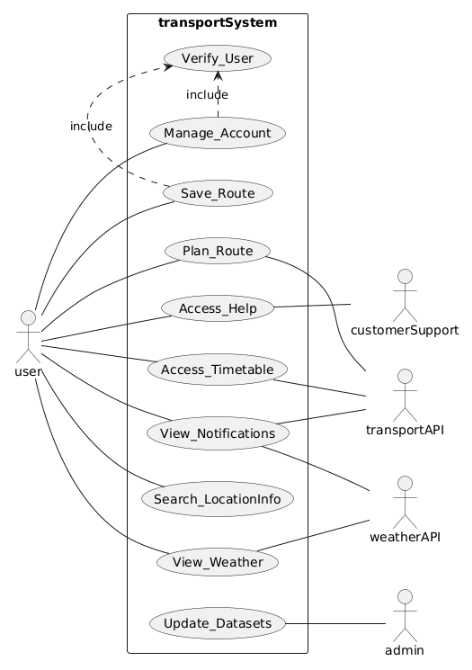
\includegraphics[width=0.35\textwidth]{images/use-case.png}
    \end{tabular}
    \caption{Use Case Diagram}
    \label{fig:UseCase}
\end{figure}
\vspace{0.5cm}

%%%%%%%%%%%%%%%%%%%%%%%%%%%%%%%%%%%%%%%%%%%%%%%%
\subsection{Design Principles}
For our project development, we will prioritize two well-known design principles: DRY (Don’t Repeat Yourself) and KISS (Keep It Simple, Stupid). Following the DRY principle will eliminate code duplication, ensuring that every piece of logic has a single responsibility within the system. We will structure our code to favour reusability, reducing overall complexity. \\ 

In alignment with the KISS principle, we will avoid unnecessary abstractions to reduce development and testing time. We will also prioritize clear, linear logic for multi-modal journey planning to ensure the system remains maintainable by both Senior and Junior Software Engineers. By keeping our design focused strictly on the defined requirements, we will minimize the likelihood of bugs and scope creep. 

%%%%%%%%%%%%%%%%%%%%%%%%%%%%%%%%%%%%%%%%%%%%%%%%

\subsection{Data Structure and Ownership}

\subsubsection{Core Domain Entities}
We decided to split the database into 2 main tables: User and Route. This is displayed in the entity relationship diagram [\ref{fig:ERD}]. We did this to separate data into meaningful sections and eliminate redundant data. This ensures whatever we produce will be smaller in size, making it more beneficial and less likely to be erroneous.  \\ \\

\begin{figure}[H]
    \centering
    \begin{tabular}{c}
        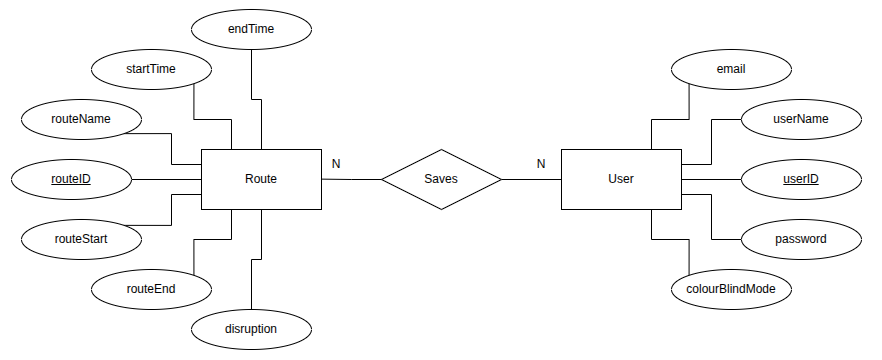
\includegraphics[width=0.65\textwidth]{images/ERD.png}
    \end{tabular}
    \caption{Entity Relationship Diagram}
    \label{fig:ERD}
\end{figure}

\subsubsection{Data Ownership Model}
The only data we will own is any account information, including emails, passwords and names. This will be the only thing we own, making it easier to keep secure. For the rest of the data, we will be using APIs, since this is easier and there are free options available. This may provide a learning curve but will provide less risk to us in the development phase of the system as well as maintenance.  
%%%%%%%%%%%%%%%%%%%%%%%%%%%%%%%%%%%%%%%%%%%%%%%%
%%%%%%%%%%%%%%%%%%%%%%%%%%%%%%%%%%%%%%%%%%%%%%%%

\subsection{External API integration}

The system integrates multiple external APIs to gather transportation information from bus services and national rail. This integration prevents data sources from being divided and the need for users to alternate between different platforms to retrieve particular information on their journey. By having multiple data sources on a single platform, it provides a reliable and user-friendly transportation experience. 

\subsubsection{API Usage}
\begin{itemize}[itemsep=2pt, topsep=4pt, parsep=0pt]
    \item \textbf{Static public transport}
    \begin{itemize}[itemsep=2pt, topsep=4pt, parsep=0pt]
        \item Providing data about stops, routes, timetables  
    \end{itemize}
    \item \textbf{Real-time public transport}
    \begin{itemize}[itemsep=2pt, topsep=4pt, parsep=0pt]
        \item Providing data on predicted arrivals, delays, cancellations 
    \end{itemize}
    \item \textbf{Weather data}
    \begin{itemize}[itemsep=2pt, topsep=4pt, parsep=0pt]
        \item Providing data on current conditions for journey area 
    \end{itemize}
\end{itemize}
\noindent
The system uses these external APIs to carry out its functionality and enhance user awareness, improve decision-making, and support safer journey planning. 

\subsubsection{Integration Approach}
Each external API has an adapter module responsible for interfacing neatly with the API and returning data from it in a clean and predictable manor. Segregating the API handling into a single controlled module results in a safer environment where errors raised are isolated from the rest of the system.

\subsubsection{Error Handling}
\begin{itemize}[label=--]
    \item API timeouts and retry mechanisms implemented.
    \item \textbf{Fault Tolerance:} Partial failures (e.g., one operator offline) do not affect the entire system.
    \item Errors logged for debugging and auditing.
\end{itemize}

\subsubsection{Security Considerations}
\begin{itemize}[label=--]
    \item Credential Security: API keys are stored securely.
    \item Data Privacy: Sensitive data is not logged.
\end{itemize}
    


%%%%%%%%%%%%%%%%%%%%%%%%%%%%%%%%%%%%%%%%%%%%%%%%
%%%%%%%%%%%%%%%%%%%%%%%%%%%%%%%%%%%%%%%%%%%%%%%%

\subsection{User Interface Design}
For this subsection, we implemented the following user interface mock-ups found in found in Appendix \ref{appendix:ui} in order to demonstrate how our project would function in process. Although this is not final, it should be a good indicator of how it will function when completed. \\

The website features a sidebar and a default screen mapping out the North West of England, which the user can pan across and zoom in on. They may click on locations in order to read information about them and plan journeys between the locations either by using the map or a search tab on the sidebar. This will open up an additional menu showing the routes between two locations, showing the method of transport with a vector as well as the time that the journey will take between the two areas. \\

Other than this, the system includes a weather tab for areas in the North West as well as a notification tab, detailing announcements about the weather in certain locations as well as any new information pertaining to travel routes that the user decides to save for convenience. \\

An account tab is also shown; when using the website for the first time, this will only request the user to log in but once done it will include the options to modify saved travel routes, update their password, log out of their personal account, or delete their personal account. Also noted are potential FAQ and Customer Support tabs that will be detailed with information on how to contact the service providers personally as well as to use other travel methods (e.g. local taxi information). 

%%%%%%%%%%%%%%%%%%%%%%%%%%%%%%%%%%%%%%%%%%%%%%%%%%%
%%%%%%%%%%%%%%%%%%%%%%%%%%%%%%%%%%%%%%%%%%%%%%%%%%%

\section{Project Milestones}
\subsection{Task List}

In the task list below, there are seven milestones:\\

\textbf{Milestone 1} involves creating the basic skeleton for the website, including user interactivity to navigate across all of the planned user interfaces, as well as making the website more accessible via colour blind mode.  \\

\textbf{Milestone 2} considers the integration of Weather and Transport APIs into the website (using a fallback mechanism so that if the site cannot update current information, it displays default routes and weather information), as well as implementing a timetable based off of transport information and allowing users to download it. \\

\textbf{Milestone 3} involves making a fully functioning account system, where users can log in and out of their personal accounts on the website while having any personal data that they have encrypted. They will also be able to delete their account or update their password. \\ 

\textbf{Milestone 4} is concerned with the functionality of route planning on the website. This will include allowing users to search, select, and sort for routes from one location to another. Multi-modal planning logic will be implemented to support buses, rail, and any combined routes between them. From there, the ability to save specific routes between places will be added to personal accounts. \\

\textbf{Milestone 5} involves the implementation of a notification alert system: this will tell users about any weather updates, as well as whether there are any disruptions to their saved routes. \\

\textbf{Milestone 6} is for the integration of map logic. The website will have map interactivity implemented so that users can zoom out and pan across a map, and there will be visualisation of travel routes implemented into the map when they are input. \\

\textbf{Milestone 7} is dedicated to the testing of the website. First, testing will be done for functional correctness of the website, then usability tests will be done after that. Finally, the user experience will be validated against accessibility and inclusivity guidelines. \\

\begin{longtable}{|p{4cm}|p{13cm}|}
\hline
\textbf{Milestone} & \textbf{Tasks} \\
\hline
\endfirsthead

\hline
\textbf{Milestone} & \textbf{Tasks} \\
\hline
\endhead

Base Website Structure 
& 
\vspace{-\topsep}
\begin{itemize}[itemsep=2pt, topsep=0pt, parsep=0pt]
    \item T1 - Develop static page structure
    \item T2 - Implement interactive elements of pages
    \item T3 - Add accessibility information
\end{itemize} \\
\hline

API Integration
& 
\vspace{-\topsep}
\begin{itemize}[itemsep=2pt, topsep=0pt, parsep=0pt]
    \item T4 - Weather API integration and fallback mechanism
    \item T5 - Transport API integration with fallback mechanism
    \item T6 - Implement timetable viewing, download logic, and dataset switching
\end{itemize} \\
\hline

Account System
& 
\vspace{-\topsep}
\begin{itemize}[itemsep=2pt, topsep=0pt, parsep=0pt]
    \item T7 - Account database implementation
    \item T8 - User account management system
\end{itemize} \\
\hline

Route Planning 
& 
\vspace{-\topsep}
\begin{itemize}[itemsep=2pt, topsep=0pt, parsep=0pt]
    \item T9 - Implement route search, selection, and sorting functionality
    \item T10 - Develop multi-modal journey planning logic
    \item T11 - Implement the ability to save routes to user accounts
\end{itemize} \\
\hline

Notification and Alert System
& 
\vspace{-\topsep}
\begin{itemize}[itemsep=2pt, topsep=0pt, parsep=0pt]
    \item T12 - Develop weather alert and notification section
    \item T13 - Develop Transport alert and notification system
\end{itemize} \\
\hline

Integration of Map Logic
& 
\vspace{-\topsep}
\begin{itemize}[itemsep=2pt, topsep=0pt, parsep=0pt]
    \item T14 - Implement map interactivity
    \item T15 - Implement visualisation of routes onto maps
\end{itemize} \\
\hline

Testing
&
\vspace{-\topsep}
\begin{itemize}[itemsep=2pt, topsep=1pt, parsep=0pt]
    \item T16 - Test function correctness for the system again the requirements stated
    \item T17 - Conduct usability tests
    \item T18 - Validate user experience against accessibility and inclusivity guidelines
\end{itemize} \\
\hline

\caption{Milestones}
\end{longtable}


%%%%%%%%%%%%%%%%%%%%%%%%%%%%%%%%%%%%%%%%%%%%%%

\subsection{Project Timeline}

The following project timeline was constructed as a guide for how long the project implementation and testing phases will take to complete. The time for task completion is based on the standard five day work week and the expected rate of working is based on the estimated difficulty of the tasks.  \\

The implementation approach we have decided to use is waterfall development. This is because our project doesn't span over a long enough time period to warrant an iterative design approach such as agile development. The key problem with this, however, is that there will be bottlenecks and dependencies in the implementation of the system where one subsystem may rely on the completion of another. We accounted for this within implementation timeline by creating a Gantt chart and an activity network for task completion based on dependencies and estimated task completion times. \\

The critical path represented by the red arrows in the activity network [\ref{fig:placeholder}] and the red tasks in the Gantt chart [\ref{fig:gantt}] have been given special consideration which is reflected in risk mitigation strategies and estimated task completion time. \\

The critical path requires the development of the page structure first, alongside its' interactivity. This is because every feature and function we create afterwards will link back and need to be implemented within the webpage. Following this, the route searching functionality needs to be implemented. This requires the UI because the user must input their start and destination point alongside filters before the routing logic can determine the routes. The route searching functionality is crucial to the system as it allows users to look at the travel routes that they may need. However, the saving of routes is not necessary to the functionality of the program, hence why it is not in the critical path. \\

The notifications for the weather and transport information will then be focused on so that users can be updated about the current conditions for any travel plans that they may have. The ability to navigate the map is then prioritised so that users can intuitively plan their journeys on the main map screen of the interface. At the end of the critical path, user testing will be done to ensure that the finished system functions as it is supposed to. \\
\begin{figure}[H]
    \centering
    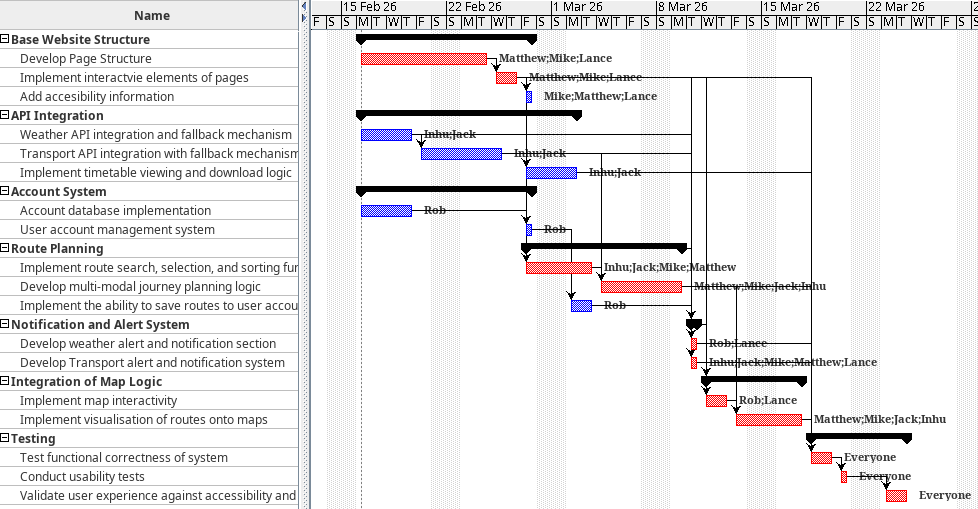
\includegraphics[width=1\textwidth]{images/gantt-chart}
    \caption{Gantt Chart}
    \caption*{\footnotesize Source: Generated using ProjectLibre \cite{projectlibre}}
    \label{fig:gantt}
\end{figure}

\begin{figure}[H]
    \centering
    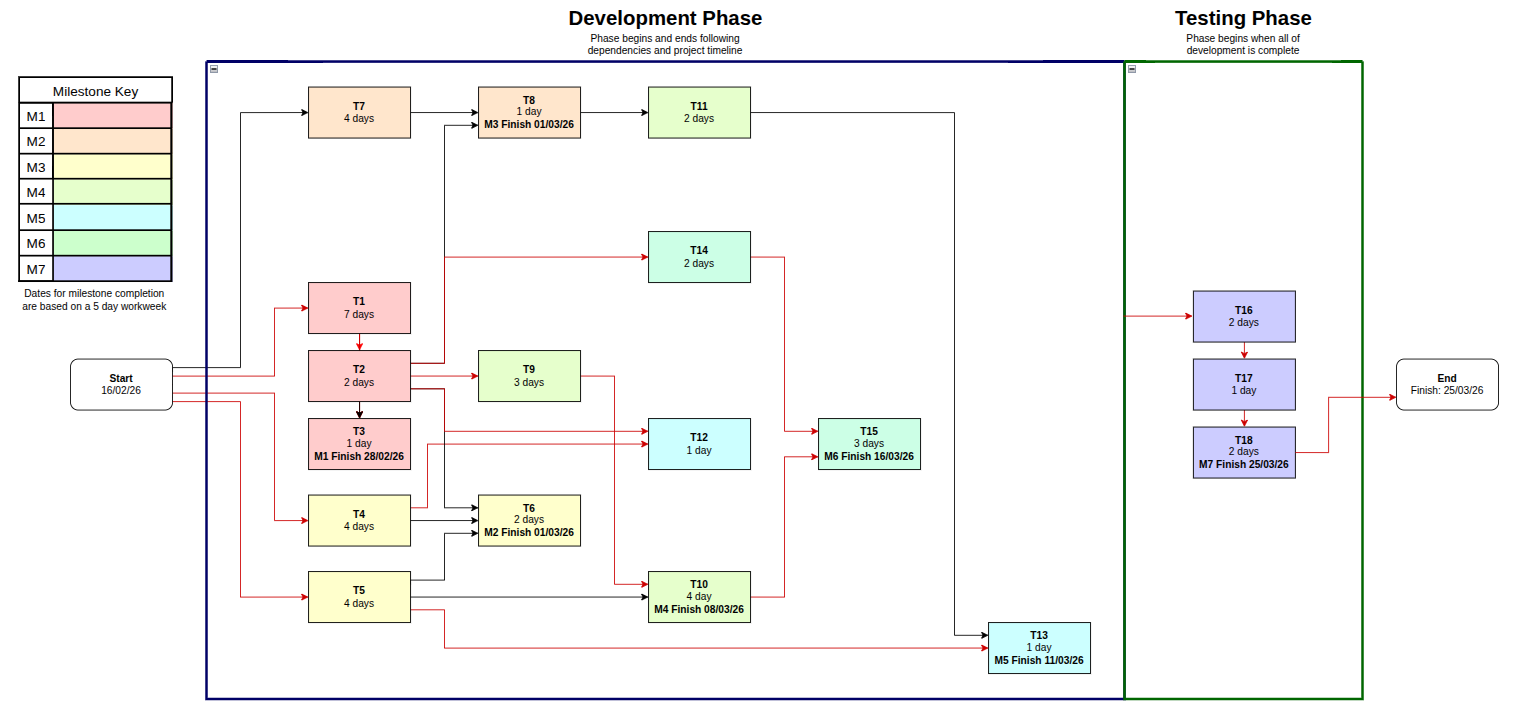
\includegraphics[width=1\linewidth]{images/activity-network}
    \caption{Activity network}
    \caption*{\footnotesize Source: Generated using draw.io \cite{drawio}}
    \label{fig:placeholder}
\end{figure}

%%%%%%%%%%%%%%%%%%%%%%%%%%%%%%%%%%%%%%%%%%%%%%%%%%%
%%%%%%%%%%%%%%%%%%%%%%%%%%%%%%%%%%%%%%%%%%%%%%%%%%%

\section{Testing Protocol}
In order to ensure the system is robust, acceptable for handover and by extension, available for use by the general public as a unified public transport navigation system, it shall be put under the scrutiny of a functional testing regime. This testing plan details how the systems features will be tested against the functional requirements and how the system will be quantitively measured against the non-functional requirements. 

\subsection*{Rationale}

Functional testing has been chosen for this system due to the rigour with which the requirements were derived from the brief and how the requirements were refined to reflect every aspect of the proposed system. 
\\
Where applicable, system tests will be designed and ran by Agentic AI workers embedded within our workflow. These workers, if at all, will exclusively be implemented where our senior software engineer deems them necessary within essential subsystems where regression could be detrimental to the project being delivered under budget and within the deadline

\begin{table}[H]
\centering
\footnotesize
\begin{tabularx}{\textwidth}{|l|X|X|X|X|}
\hline
\textbf{ID} & \textbf{Test Scenario} & \textbf{Req.} & \textbf{Steps} & \textbf{Expected Results} \\
\hline

TC1 &
Plan a multi-modal, multi-operator journey with disruption handling &
FR1, FR2, FR3, FR4, FR7, FR9 &
\begin{enumerate}[nosep,leftmargin=*]
\item Open journey planner.
\item Set origin to bus-only stop in Blackpool.
\item Set destination to Lancaster.
\item Choose time requiring bus + rail.
\item Generate options.
\item Simulate delay/cancellation and refresh.
\end{enumerate}
&
\begin{itemize}[nosep,leftmargin=*]
\item Bus + rail legs shown (FR1).
\item Multiple operators shown (FR2).
\item Scheduled times shown (FR3).
\item Live updates shown (FR4).
\item Disruption alerts + alternatives (FR7).
\item Routes switchable (FR9).
\end{itemize}
\\
\hline

TC2 &
Explore stops/stations via interactive map &
FR8, FR14, FR3, FR4, FR12 &
\begin{enumerate}[nosep,leftmargin=*]
\item Open map.
\item Click rail station.
\item Click nearby bus stop.
\end{enumerate}
&
\begin{itemize}[nosep,leftmargin=*]
\item Details panel appears (FR14).
\item Panel updates on selection.
\item Departures shown (FR3).
\item Live info shown/marked unavailable (FR4).
\item Accessibility shown (FR12).
\item Map visualisation correct (FR8).
\end{itemize}
\\
\hline

TC3 &
Plan journey and view weather &
FR1, FR3, FR9, FR10 &
\begin{enumerate}[nosep,leftmargin=*]
\item Open planner.
\item Plan journey.
\item Open details.
\item View weather.
\end{enumerate}
&
\begin{itemize}[nosep,leftmargin=*]
\item Weather displayed (FR10).
\item Journey options returned (FR1).
\item Timetable available (FR3).
\item Routes modifiable (FR9).
\end{itemize}
\\
\hline

TC4 &
First-time usability and accessibility &
NFR6, NFR7, NFR9 &
\begin{enumerate}[nosep,leftmargin=*]
\item First-time user completes tasks.
\item Enable colour-blind mode.
\item Confirm no excess data collection.
\end{enumerate}
&
\begin{itemize}[nosep,leftmargin=*]
\item Tasks completed with minimal confusion (NFR6).
\item Colour-blind mode clear (NFR7).
\item No unnecessary data stored (NFR9).
\end{itemize}
\\
\hline

TC5 &
Ethical handling of evaluation &
NFR14, NFR9 &
\begin{enumerate}[nosep,leftmargin=*]
\item Conduct evaluation.
\item Provide study info.
\item Obtain consent.
\item Store results anonymously.
\end{enumerate}
&
\begin{itemize}[nosep,leftmargin=*]
\item Consent obtained.
\item Data anonymised and minimal.
\end{itemize}
\\
\hline

TC6 &
Core function during feed failure &
NFR3, NFR13 &
\begin{enumerate}[nosep,leftmargin=*]
\item Simulate feed outage.
\item Plan journey + open board.
\item Restore feed.
\item Inspect logs.
\end{enumerate}
&
\begin{itemize}[nosep,leftmargin=*]
\item Core functions continue (NFR3).
\item No crash/blank screen.
\item Failure/recovery logged (NFR13).
\end{itemize}
\\
\hline

\end{tabularx}
\caption{Test Case Register}
\end{table}



\newpage

%%%%%%%%%%%%%%%%%%%%%%%%%%%%%%%%%%%%%%%%%%%%%%%%%%%
%%%%%%%%%%%%%%%%%%%%%%%%%%%%%%%%%%%%%%%%%%%%%%%%%%%

\section{Risk Management}

%%%%%%%%%%%%%%%%%%%%%%%%%%%%%%%%%%%%%%%%%%%%%%%%%%%
%%%%%%%%%%%%%%%%%%%%%%%%%%%%%%%%%%%%%%%%%%%%%%%%%%%

\subsection{Risk Scoring}
Risks are evaluated based on likelihood and impact using a 5-point scale.
The overall risk rating is determined by multiplying likelihood and impact scores.

\begin{itemize}[itemsep=2pt, topsep=4pt, parsep=0pt]
    \item Likelihood: Very Low (1) to Very High (5)
    \item Impact: Very Low (1) to Very High (5)
\end{itemize}

%%%%%%%%%%%%%%%%%%%%%%%%%%%%%%%%%%%%%%%%%%%%%%%%%%%%
%%%%%%%%%%%%%%%%%%%%%%%%%%%%%%%%%%%%%%%%%%%%%%%%%%%%

\subsection{Risk Register}
\begin{table}[h]
\centering
\begin{tabular}{|l|p{4cm}|c|c|p{8cm}|}
\hline
\textbf{ID} & \textbf{Risk Description} & \textbf{Likelihood} & \textbf{Impact} & \textbf{Mitigation Strategy} \\
\hline
R-01 & Staff Sickness & (4) & (3) & Allowances in the budget for contractors, coupled with thorough documentation allowing for employees to be brought up to speed efficiently \\

\hline

R-02 & Resource Exhaustion & (2) & (5) & Thorough management and predictions of resource usage with researched justifications and overhead accountants \\

\hline

R-03 & Improper or insufficient testing & (2) & (4) & In place will be a detailed test design programme as well as a strict protocol for acceptance which we must meet all criteria for prior to acceptance from stakeholders \\

\hline

R-04 & Cloud service instability or outages & (2) & (5) & Only reputable services are used, with backup services researched in case the project requires a different service to be used \\

\hline

R-05 & Project length exceeding time frame & (2) & (3) & Scope of the project is strictly defined as well as contingencies in budget for contractors to be brought on to assist in critical path development if we fall behind the schedule \\

\hline

R-06 & Scope creep during development & (4) & (4) & Thorough definitions of what comprises the project scope as well as explicit notes as to what the project is not involved with \\

\hline

R-07 & Poor cyber security practices leaving our system(s) vulnerable & (2) & (5) & Using latest industry standards to protect our services \\

\hline

R-08 & Non-compliance with data protection or ethical requirements & (2) & (5) & Minimise personal data collection, follow ethical guidance, and document consent processes  \\

\hline

R-09 & System performance degrades under increased user load & (3) & (4) & Optimise query handling and limit resource-intensive operations; define performance thresholds  \\

\hline

R-10 & External transport API data quality issues & (4) & (4) & Validate incoming data, cross-check where possible, and clearly indicate data limitations to users  \\

\hline

R-11 & Over-reliance on Agentic AI & (3) & (4) & The prompts used for AI will be planned and reviewed by multiple developers. Code produced by AI will also be reviewed and tested, and documentation will be produced alongside any code. \\

\hline

R-12 & Failure to integrate subsystems  & (3) & (5) & Define clear interfaces early, integrate incrementally, and test integrations frequently  \\

\hline
\end{tabular}
\caption{Project Risk Register}
\end{table}

\newpage

%%%%%%%%%%%%%%%%%%%%%%%%%%%%%%%%%%%%%%%%%%%%%%%%%%%%%%%%
%%%%%%%%%%%%%%%%%%%%%%%%%%%%%%%%%%%%%%%%%%%%%%%%%%%%%%%%

\subsection{Risk Matrix}

\begin{table}[h]
\centering
\renewcommand{\arraystretch}{1.6}
\begin{tabular}{|c|c|c|c|c|c|}
\hline
\textbf{Impact} $\backslash$ \textbf{Likelihood}
& \textbf{Very Low}
& \textbf{Low}
& \textbf{Medium}
& \textbf{High}
& \textbf{Very High} \\
\hline
\textbf{Very High}
& \cellcolor{yellow!40}
& \cellcolor{orange!50} R-02, R-04, R-07, R-08
& \cellcolor{red!60} R-12
& \cellcolor{red!80}
& \cellcolor{red!90} \\
\hline
\textbf{High}
& \cellcolor{yellow!30}
& \cellcolor{yellow!60} R-03
& \cellcolor{orange!60} R-09, R-11
& \cellcolor{red!70} R-06, R-10
& \cellcolor{red!80} \\
\hline
\textbf{Medium}
& \cellcolor{green!30}
& \cellcolor{yellow!30} R-05
& \cellcolor{yellow!50}
& \cellcolor{orange!60} R-01
& \cellcolor{red!70} \\
\hline
\textbf{Low}
& \cellcolor{green!20}
& \cellcolor{green!30}
& \cellcolor{yellow!30}
& \cellcolor{yellow!50}
& \cellcolor{orange!60} \\
\hline
\textbf{Very Low}
& \cellcolor{green!10}
& \cellcolor{green!20}
& \cellcolor{green!30}
& \cellcolor{yellow!30}
& \cellcolor{yellow!40} \\
\hline
\end{tabular}
\caption{Risk Matrix with Embedded Risk Identifiers}
\end{table}

%%%%%%%%%%%%%%%%%%%%%%%%%%%%%%%%%%%%%%%%%%%%%%%%%%%
%%%%%%%%%%%%%%%%%%%%%%%%%%%%%%%%%%%%%%%%%%%%%%%%%%%

\section{Project Budget}

This section presents a transparent and internally consistent financial 
model for the proposed three-month development phase including a year of off-site technician support. All costs are categorised to avoid duplication between labour burden and project-specific operational expenditure.

%%%%%%%%%%%%%%%%%%%%%%%%%%%%%%%%%%%%%%%%%%%%%%%%%%%%%%%%
%%%%%%%%%%%%%%%%%%%%%%%%%%%%%%%%%%%%%%%%%%%%%%%%%%%%%%%%

\subsection{Base Wages}

Hourly wage rates were derived from the Indeed Salary Calculator (UK) \cite{indeed2025} 
and converted from annual salary estimates to hourly rates assuming 1,800 
billable hours per annum. Included in this is support from a help desk technician for one calendar year after the project has been delivered. 


\begin{table}[h]
\centering
\begin{tabular}{|l|c|r|}
\hline
\textbf{Cost Component} & \textbf{Detail} & \textbf{Amount (£)} \\
\hline
Senior Engineering Manager & 150 hrs @ £72.97/hr & 10,945.50 \\
Senior Software Engineer & 150 hrs @ £37.15/hr & 5,572.50 \\
Junior Software Engineers (4) & 150 hrs @ £17.96/hr each & 10,776.00 \\
Software Testers & 30 hrs @ £29.20/hr & 876.00 \\
Quality Assurance Analyst & 30 hrs @ £17.25/hr & 517.50 \\
Help Desk Technician & 2,080 hrs @ £17.00/hr & 35,360.00 \\
\hline
\textbf{Total Base Wages} & -- & \textbf{64,023.50} \\
\hline
\end{tabular}
\caption{Base wage allocation by role}
\end{table}

%%%%%%%%%%%%%%%%%%%%%%%%%%%%%%%%%%%%%%%%%%%%%%%%%%%%%%%%%%%%
\subsection{Employment Burden and Productivity Adjustments}

\subsubsection*{Statutory and Organisational Burden (28.8\%)}

The employment burden rate incorporates statutory employer costs and 
core organisational overhead allocation:

\begin{itemize}[itemsep=2pt, topsep=4pt, parsep=0pt]
    \item Employer National Insurance: 13.8\%
    \item Minimum employer pension contribution: 3\%
    \item Organisational support allocation (HR, IT support, finance, management oversight): 12\%
\end{itemize}

\[
13.8\% + 3\% + 12\% = 28.8\%
\]

\subsubsection*{Productivity and Workforce Risk Adjustment (25\%)}

An additional adjustment accounts for non-billable time and workforce risk:

\begin{itemize}[itemsep=2pt, topsep=4pt, parsep=0pt]
    \item Statutory leave and non-billable time: 12\%
    \item Training and skills development: 3\%
    \item Equipment and software provisioning: 4\%
    \item Absence and attrition risk allowance: 6\%
\end{itemize}

\[
12\% + 3\% + 4\% + 6\% = 25\%
\]

\begin{table}[h]
\centering
\begin{tabular}{|l|r|}
\hline
\textbf{Cost Component} & \textbf{Amount (£)} \\
\hline
Fully loaded labour subtotal & 82,462.27 \\
Productivity and workforce adjustment (25\%) & 20,615.57 \\
\hline
\textbf{Total Employee Cost} & \textbf{103,077.84} \\
\hline
\end{tabular}
\caption{Total employment cost after burden and productivity adjustments}
\end{table}

%%%%%%%%%%%%%%%%%%%%%%%%%%%%%%%%%%%%%%%%%%%%%%%%%%%%%%%%%%%%
\subsection{Project-Specific Non-Labour Costs}

This subsection details the project-specific non-labour costs required to deliver and support the proposed system. These costs represent operational and enabling expenditures that are not already incorporated within the employment burden model outlined in Section~8.2. All figures are derived using identifiable cost drivers where possible (e.g., team size, project duration, subscription structure, or defined risk allowance) in order to avoid duplication and ensure transparency of assumptions. \\

Costs are intentionally separated from core salary overheads to distinguish between baseline organisational expenditure and project-dependent operational requirements such as facilities, hosting infrastructure, governance activity, deployment, and contractor risk mitigation. This separation ensures that non-labour expenditure reflects only the incremental costs necessary for project execution and one year of post-delivery support.


\subsubsection*{Facilities Allocation}

Dedicated workspace is derived using a driver-based model:

\[
\text{Rent} = (\text{team size} \times \text{m}^2/\text{person}) 
\times (\pounds/\text{m}^2/\text{month}) \times (\text{months})
\]

Using:
\[
10 \times 4.9 \times 130 \times 3 \approx 19,200
\]

\begin{table}[h]
\centering
\begin{tabular}{|l|r|}
\hline
\textbf{Cost Component} & \textbf{Amount (£)} \\
\hline
Project facilities (3 months) & 19,200.00 \\
Cloud hosting & 3,000.00 \\
Software licences & 1,832.84 \\
Travel and stakeholder engagement & 2,500.00 \\
Governance and reporting & 4,000.00 \\
Deployment and handover & 3,500.00 \\
Contractor contingency allowance & 11,000.00 \\
\hline
\textbf{Total Non-Labour Cost} & \textbf{45,032.84} \\
\hline
\end{tabular}
\caption{Project-specific operational costs (no duplication of labour overhead)}
\end{table}

%%%%%%%%%%%%%%%%%%%%%%%%%%%%%%%%%%%%%%%%%%%%%%%%%%%%%%%%%%%%
\subsection{Contingency Allowance}

A contingency reserve equivalent to 10\% of subtotal (excluding VAT) 
is applied to mitigate financial and schedule risk exposure.

\[
(103,077.84 + 45,032.84) \times 0.10 = 14,811.07
\]

%%%%%%%%%%%%%%%%%%%%%%%%%%%%%%%%%%%%%%%%%%%%%%%%%%%%%%%%%%%%
\subsection{Full Project Cost Including VAT}

\begin{table}[H]
\centering
\begin{tabular}{|l|r|}
\hline
\textbf{Cost Component} & \textbf{Amount (£)} \\
\hline
Total employee cost & 103,077.84 \\
Total non-labour cost & 45,032.84 \\
Contingency (10\%) & 22,216.60 \\
\hline
Subtotal (excl. VAT) & 170,327.28 \\
VAT (20\%) & 34,065.46
 \\
\hline
\textbf{Total Project Cost (incl. VAT)} & \textbf{204,392.74} \\
\hline
\end{tabular}
\caption{Consolidated financial summary}
\end{table}

\noindent
This subsection consolidates the full financial implications of the project by aggregating labour costs, non-labour expenditures, and contingency provision, prior to the application of Value Added Tax (VAT). Direct labour costs are derived from role-specific hourly rates and allocated working hours and are subsequently adjusted to reflect true employment costs through the inclusion of statutory contributions, benefits, training, equipment, productivity losses, and allowances for staffing risk. This approach ensures that personnel-related expenditure represents the full organisational cost rather than nominal wages alone. \\

Non-labour costs account for all operational and delivery-supporting expenditures required to enable project execution, including infrastructure, software licensing, administrative overheads, governance activities, deployment, documentation, and fixed facilities costs. A contingency allowance equivalent to 10\% of the pre-VAT subtotal is applied to mitigate financial uncertainty and potential schedule-related risks. \\

The resulting subtotal, exclusive of VAT, provides a transparent and defensible estimate of baseline project expenditure. The subsequent application of VAT at the prevailing rate of 20\% yields a total project cost of \pounds204{,}392.74 \\

\section{AI Use Declaration}
\begin{table}[H]
    \centering
    \begin{tabular}{|l|p{2cm}|p{5cm}|p{6cm}|}
    \hline
         \textbf{Section} & \textbf{Tool used} & \textbf{How was it used} & \textbf{How was the output verified} \\
         \hline
         User Interface Design & Copilot & Used it to write an alluring description for the city of Blackpool, which is supposed to be accessible by clicking the city of Blackpool on the map that makes up the main interface. & One of our group member is from Blackpool and can verify that everything said in the paragraph is factual to the city. \\
         \hline
         General & Overleaf & Used AI grammar tools to correct across whole document. & The grammar was corrected to perfect English. \\
    \hline
    \end{tabular}

\end{table}

We declare that we have used Artificial Intelligence tools only as described above. All submitted work reflects my own understanding, and I take full responsibility for its accuracy and integrity. 

\newpage

\bibliographystyle{plain}
\bibliography{references}

\newpage

\section{Appendix}


\subsection{UI Mock-ups}\label{appendix:ui} 
The UI mock-ups designed to show how the interface will appear to users \\
\vspace{0.5cm}
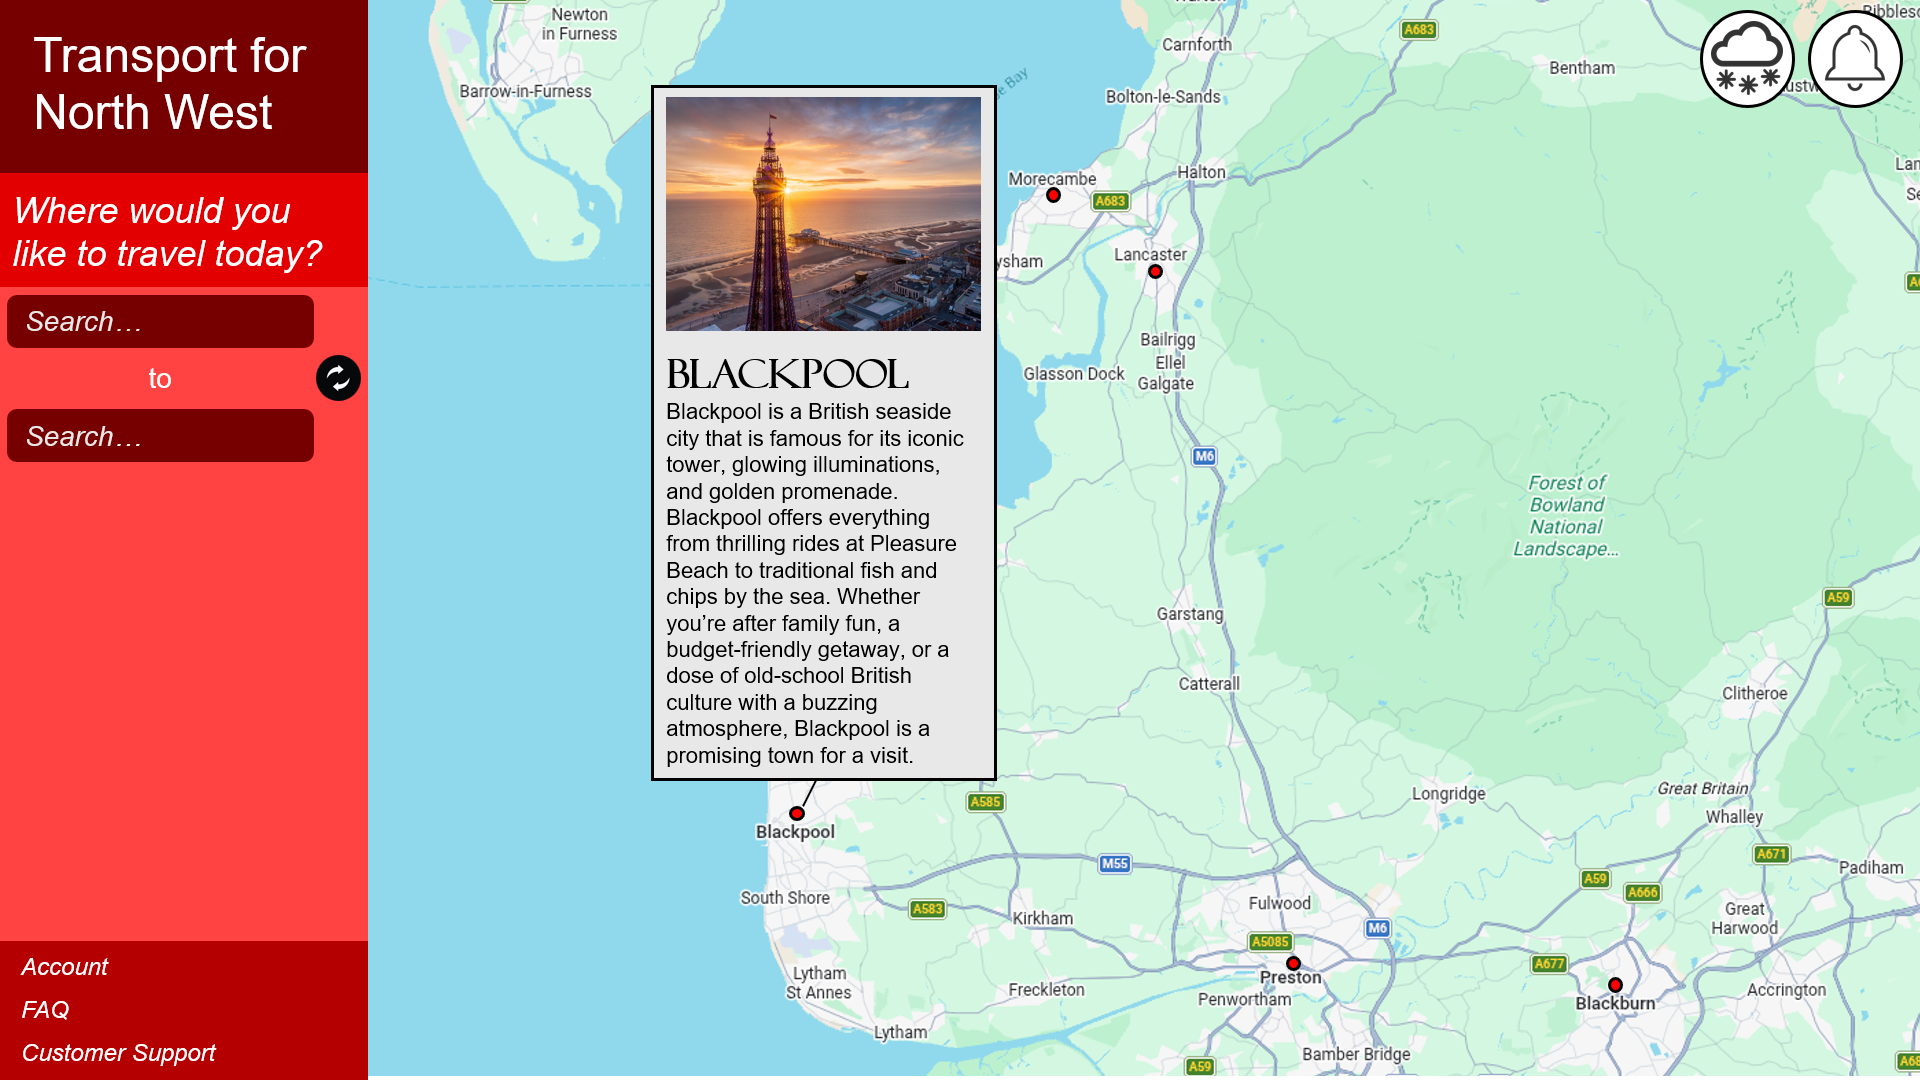
\includegraphics[width=1\textwidth]{images/ui-mock-ups/ui-1.png}\label{appendix:ui-main-view}
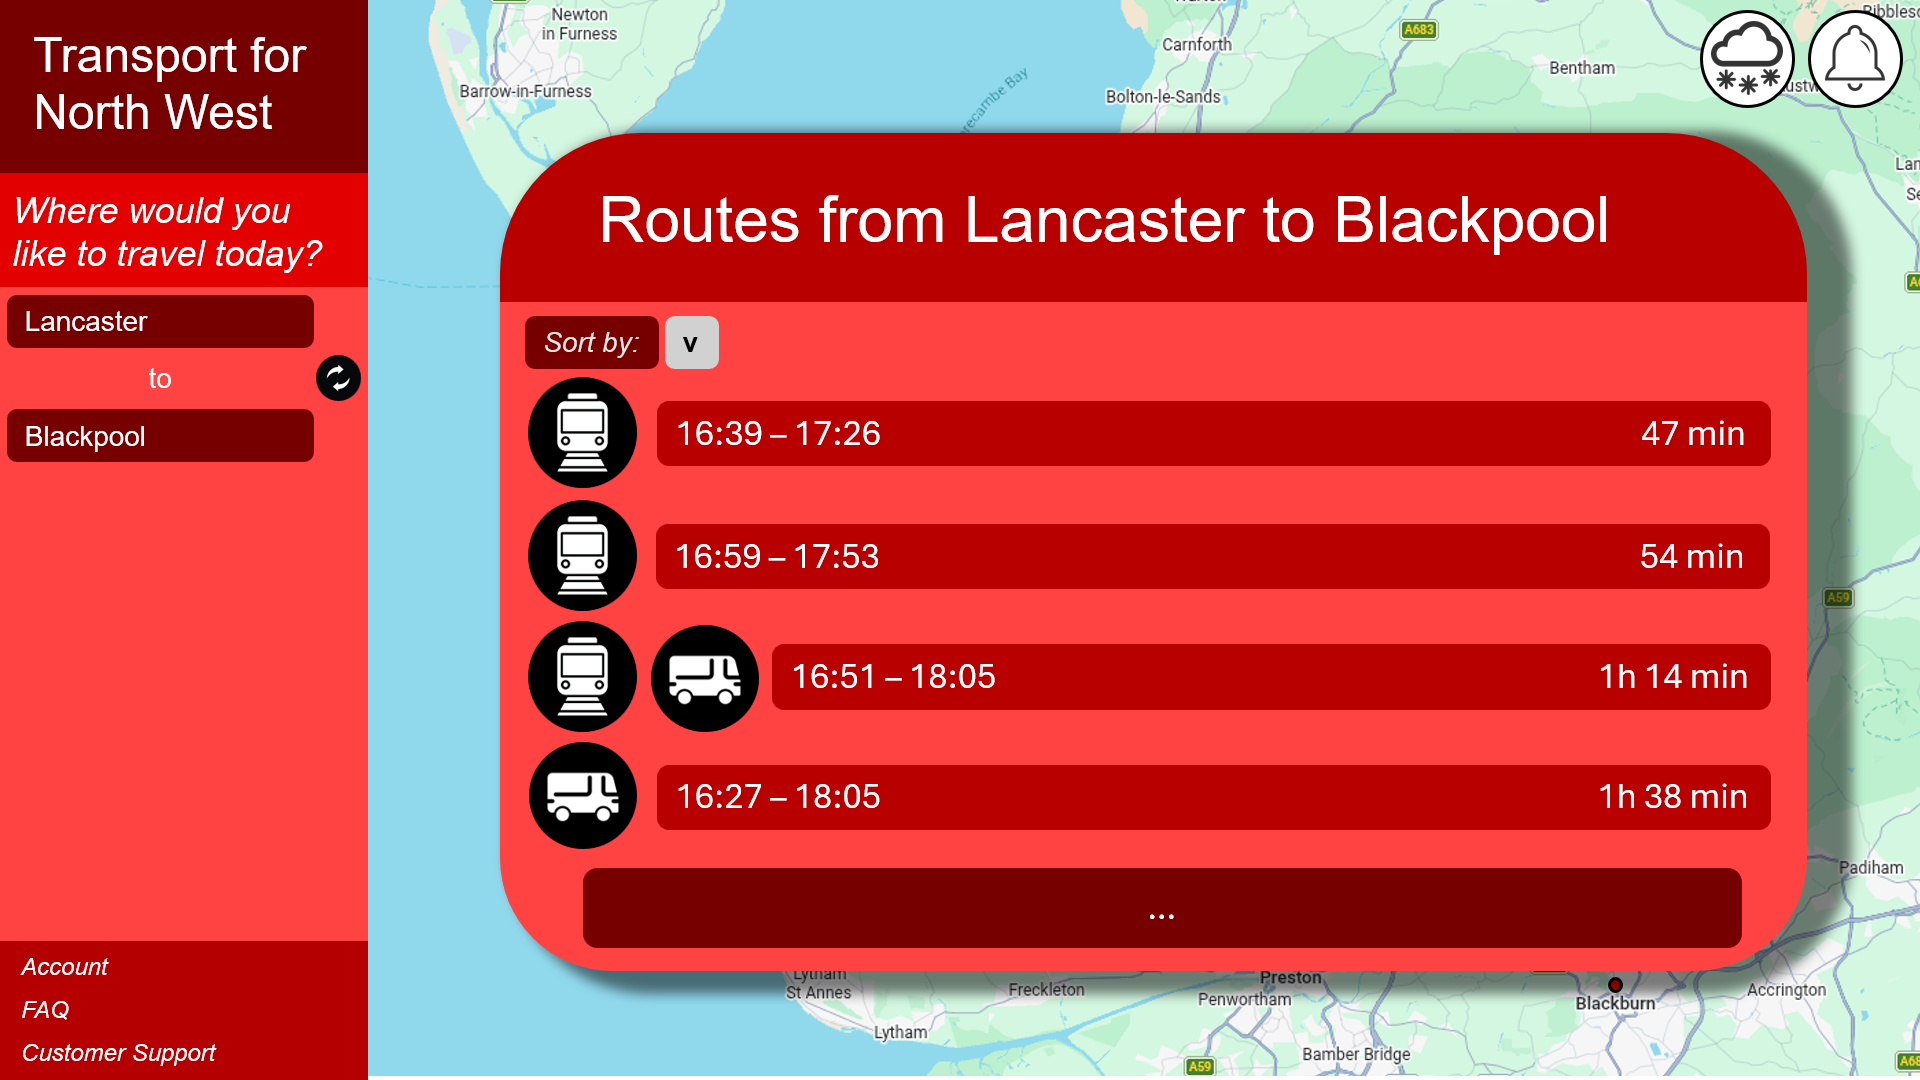
\includegraphics[width=1\textwidth]{images/ui-mock-ups/ui-2.png}\label{appendix:ui-route-selctor}
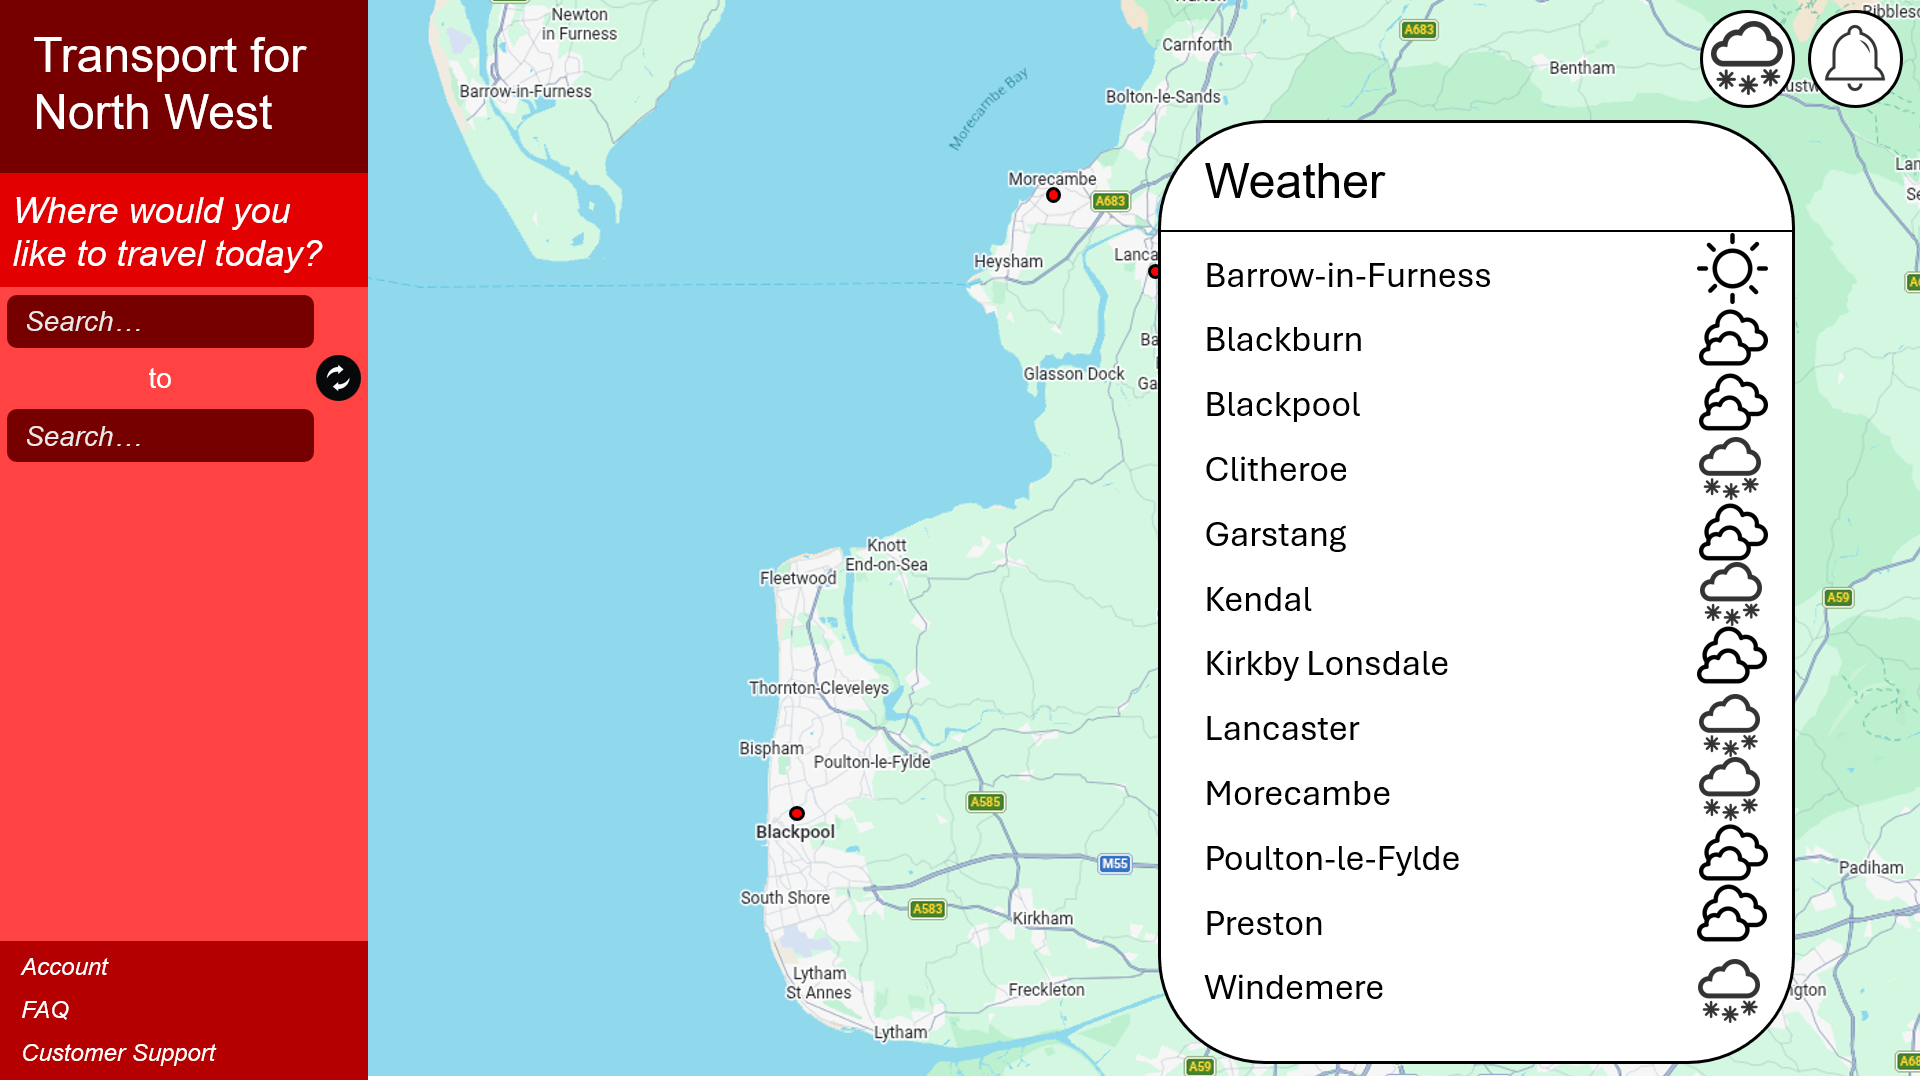
\includegraphics[width=1\textwidth]{images/ui-mock-ups/ui-3.png}\label{appendix:ui-weather}
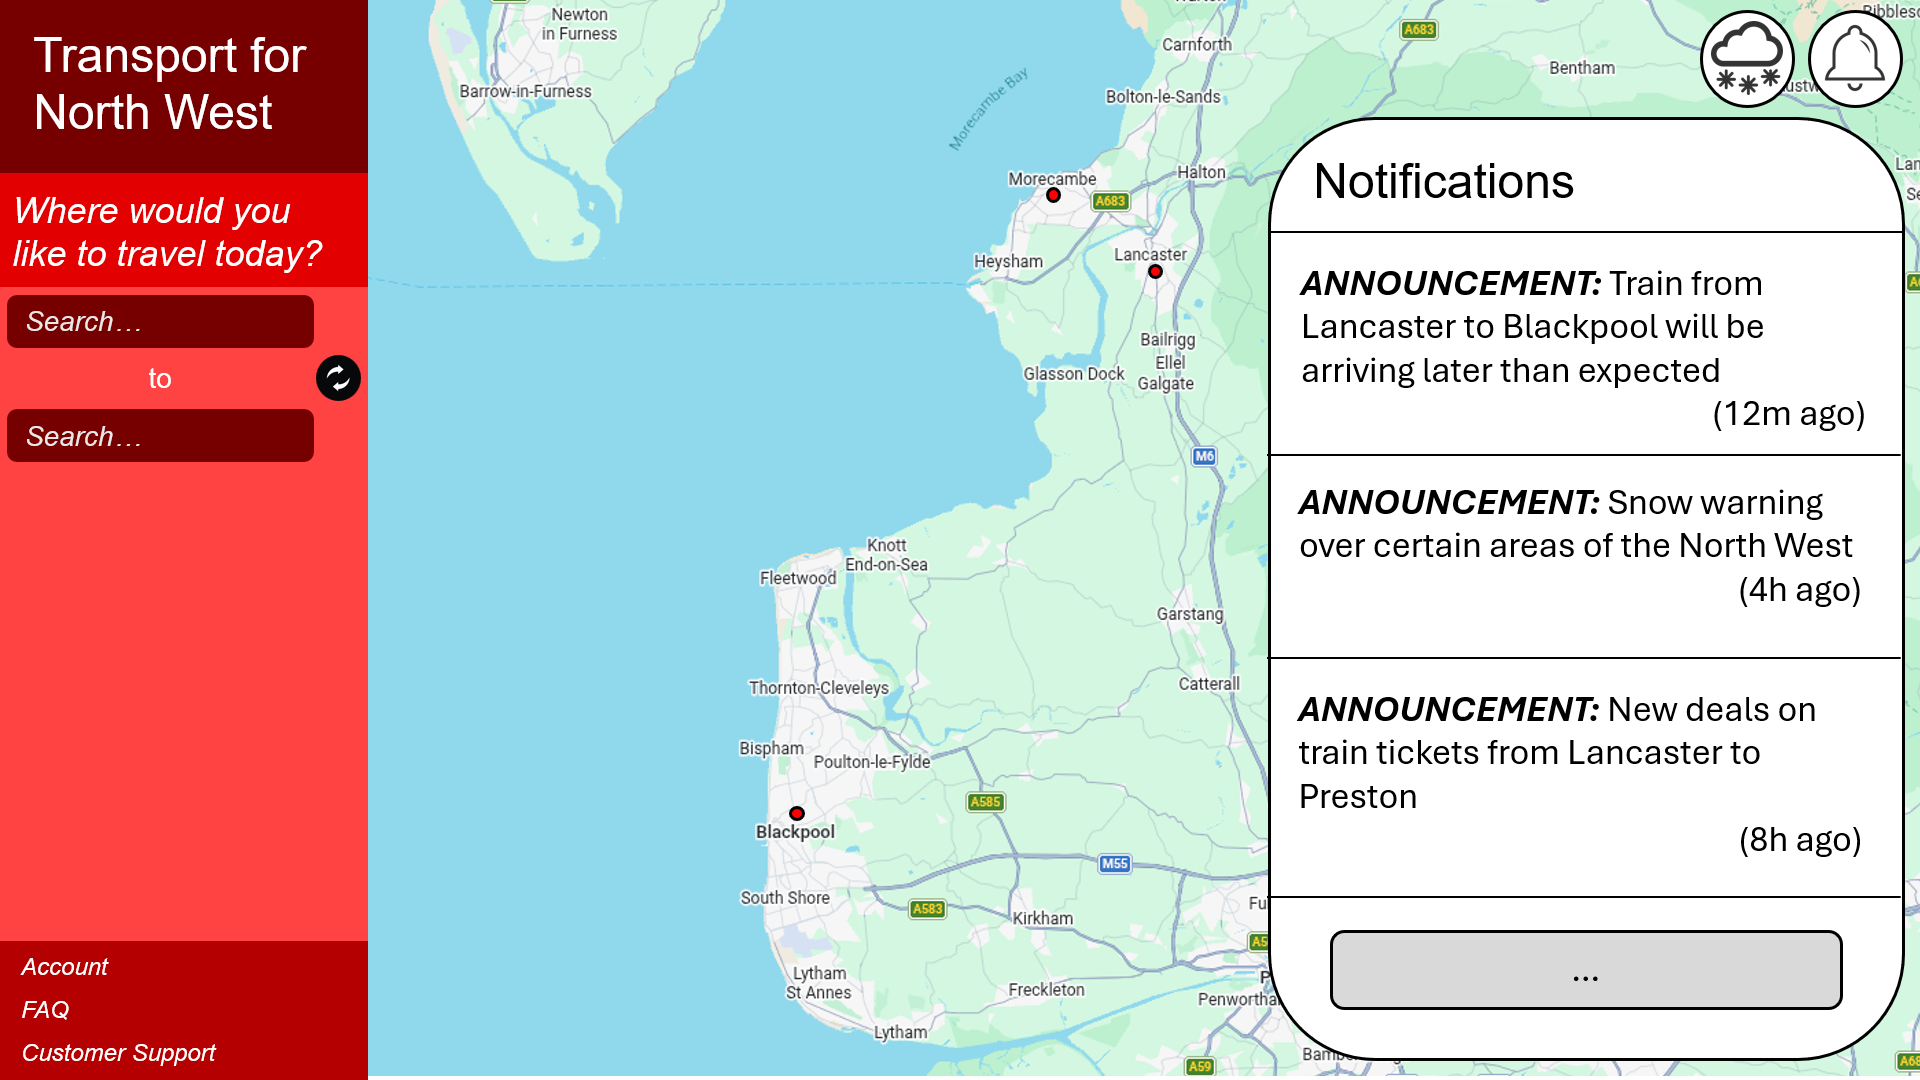
\includegraphics[width=1\textwidth]{images/ui-mock-ups/ui-4.png}\label{appendix:ui-alert-system}
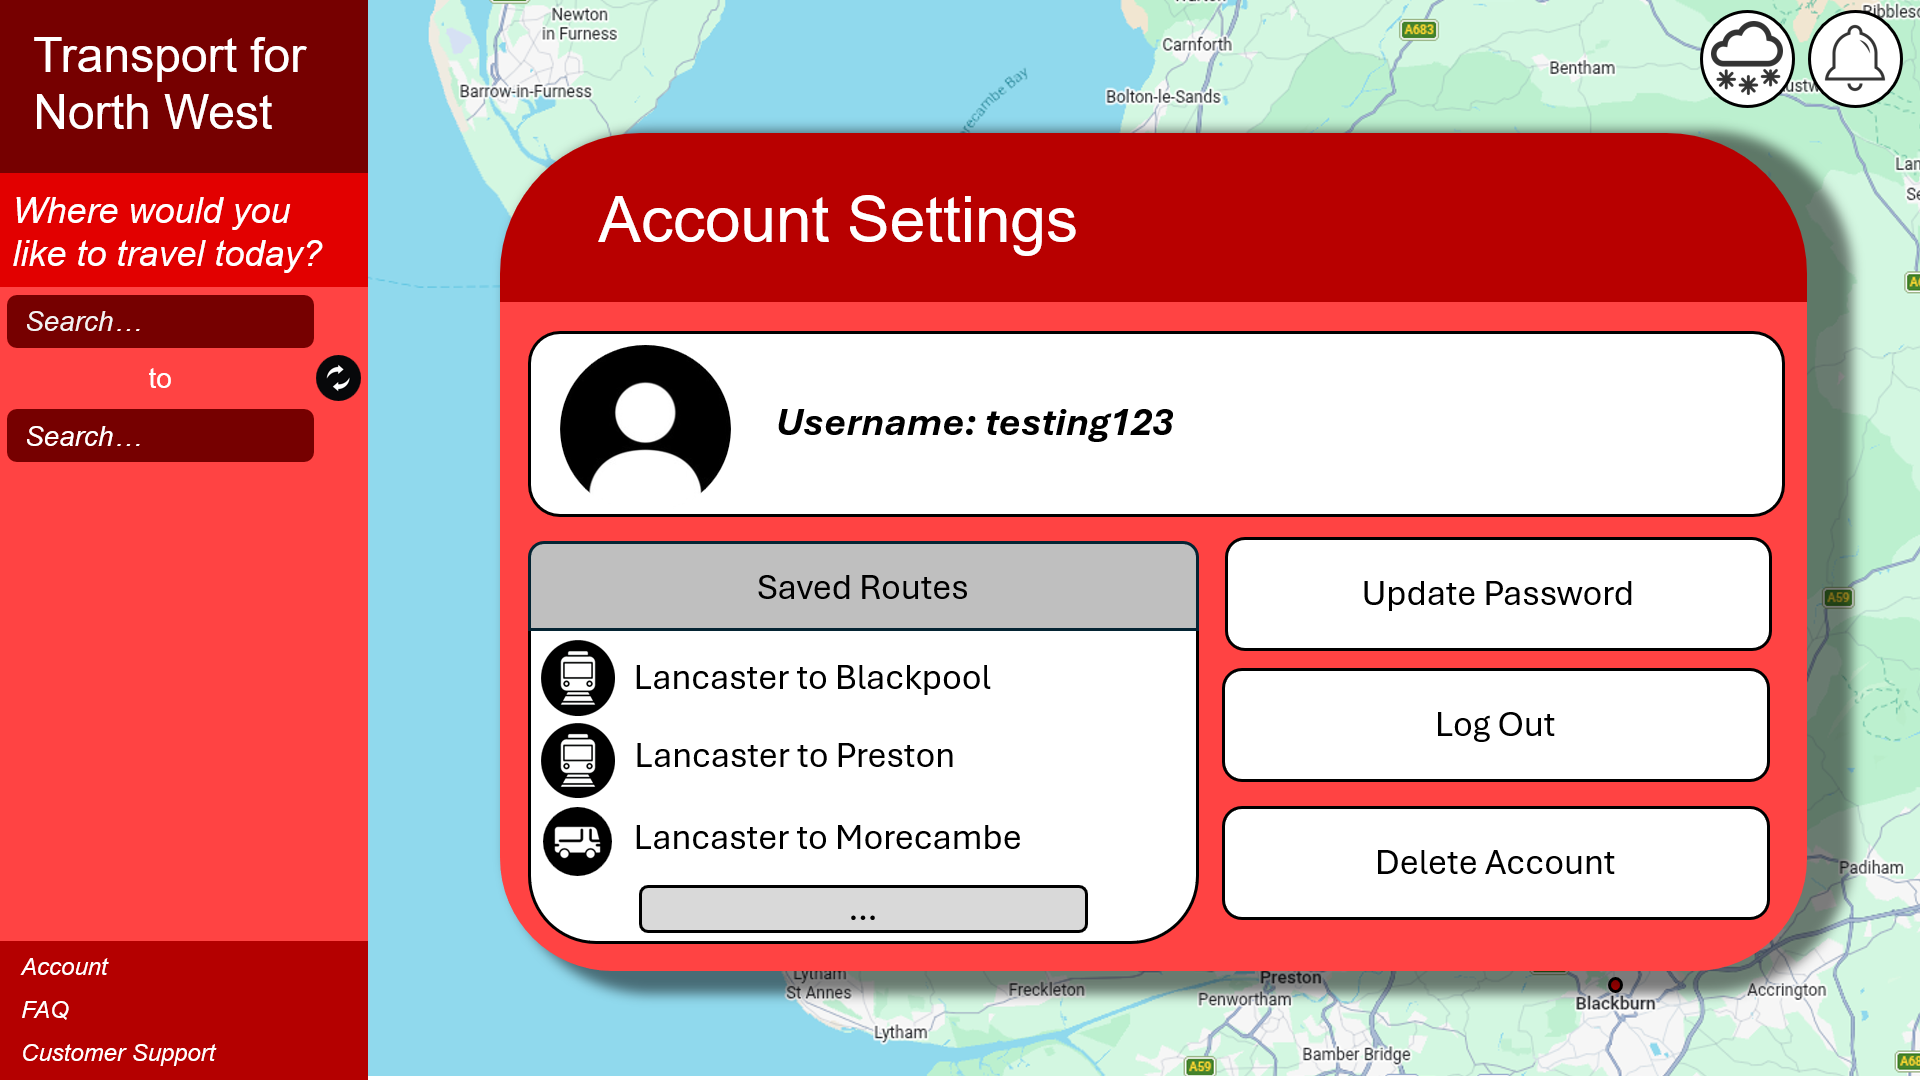
\includegraphics[width=1\textwidth]{images/ui-mock-ups/ui-5.png}\label{appendix:ui-account-management}


%%%%%%%%%%%%%%%%%%%%%%%%%%%%%%%%%

\end{document}
